\documentclass[12pt]{article}
\usepackage[czech]{babel}
\usepackage[utf8]{inputenc}
\usepackage[plainpages=false,pdfpagelabels,unicode]{hyperref}
\usepackage[pdftex]{graphicx}
\usepackage[margin=2cm, includefoot]{geometry}

\begin{document}

\title{Experimentálne metody a špeciálne praktikum \\
Langmuirová sonda}
\author{Pavel Ondračka a Roman Petráš}
\maketitle

\section{Teorie}
Sondou všeobecne rozumieme vodič malých rozmerov vnorení do plazmy za účelom zistenia nejakej fyzikálnej veličiny. Najčastejšie sa používajú vodiče tvaru doštičky, valca a gule. Sondy môžeme podľa počtu elektród zaradiť medzi jednoduché a dvojité. Počas nášho merania sme pracovali s~jednoduchou sondou v tvare valca s dĺžkou 1\,cm a polomerom 0,19\,mm (s povrchom 1,194.10$^{-5}$\,m$^2$). Meraním prúdu a napätia na sonde dostaneme sondovú charakteristiku, ktorú môžeme rozdeliť na~časti podľa dominancie dopadajúcich častíc. Pokiaľ dominuje iónový prúd, sonda je na~zápornom potenciáli oproti plazme. Pri menších hodnotách záporného potenciálu začínajú na~sondu dopadať aj rýchle elektróny, kým nedôjde k~vyrovnaniu prúdov. Tok elektrónov na sondu sa pri~ďalšom vzraste napätia stáva dominantný. Ak je sonda kladná vzhľadom k~plazmovému potenciálu, do\-chádza k~odpudzovaniu iónov a priťahovaniu elektrónov, sledujeme tak nasýtený elektrónový prúd.

Pre oblasti nasýtených prúdov, môžeme prúd vyjadriť pomocou vzťahu
\begin{equation}
I=eA \frac{n_\mathrm{e} \bar{v}}{4} \left(1 - \frac{e U}{k T}\right)^{\frac{1}{2}} \, \mathrm{,}
\end{equation}
kde $A$ je plocha sondy, $e$ elementárny náboj, $T$ teplota elektrónov a $\bar{v}$ je stredná aritmetická rýchlosť elektrónov.

Zo smernice $k_\mathrm{n}$ grafu $I^2 = f(U)$ môžeme určiť koncentráciu elektrónov v oblasti nasýtených prúdov
\begin{equation}
n_\mathrm{e} = \frac{1}{eA}\sqrt{\frac{2 k_\mathrm{n} \pi m}{e}} \, \mathrm{.}
\end{equation}

Pomocou Langmuirovej bez zrážkovej teórie sondového prúdu, kde sa uvažuje maxwellovské rozdelenie rýchlosti elektrónov za nízkych tlakov, môžeme prúd v intervale $(U_\mathrm{f} , U_p)$ vyjadriť

\begin{equation}
I=eA \frac{n_\mathrm{e} \bar{v}}{4} \, \mathrm{exp}\left(\frac{e U}{k T}\right) \, \mathrm{.}
\end{equation}

Zo smernice $k_T$ závislosti $\mathrm{ln} I = f(U)$ určíme teplotu elektrónov vzťahom

\begin{equation}
T = \frac{e}{k_T k} \, \mathrm{.}
\end{equation}

V prípade rovnosti potenciálu sondy s plazmovým, pozorujeme elektrónový a iónový prúd, pričom platí $\Delta U = U_\mathrm{s} - U_p = 0$.

V tejto oblasti môžeme určiť koncentráciu elektrónov ako

\begin{equation}
n_\mathrm{e} = \frac{I}{eA}\sqrt{\frac{2 \pi m}{k T}} \, \mathrm{.}
\end{equation}

Pokiaľ graf závislosti $\mathrm{ln} I = f(U)$ nie je lineárni, rozdelenie elektrónov nie je maxwellovské. V takom prípade určíme rozdeľovaciu funkciu pomocou Druyvesteinovej teórie z druhej derivácie prúdu

\begin{equation}
f(e|U|)= \frac{2 \sqrt{2 m |U|}}{e^{5/2} A} \frac{d^2 I}{dU^2}
\end{equation}

Koncentráciu elektrónov potom určíme ako integrál z rozdeľovacej funkcie od nuly do nekonečna.

\subsection{Kompenzovaná Langmuirova sonda}

Vysokofrekvenčne kompenzovaná sonda je umiestnená nad stredom reaktoru a je posúvatelná vo~vodorovnom smere. Sondu tvorí volfrámový valcový drôt. Sonda je vybavená referenčnou a kompenzačnou elektródou. Kompenzačná elektróda je so sondou prepojená na obvod, ktorý obsahuje dva rezonančné obvody kondenzátorov a cievok, ktoré sú naladené na frekvenciu prítomného poľa a prípadne vyššej harmoniky. Táto elektróda sleduje frekvenciu prítomného poľa, vďaka ktorej je sonda vysokofrekvenčne kompenzovaná. Referenčná elektróda sleduje fluktuácie v plazme.

\section{Měření}
Voltampérové charakteristiky sondy byly měřeny pro 10 různých tlaků v reaktoru, na obrázku \ref{VA} jsou zobrazen jejich průběhy (pro přehlednost jsou v grafu vykresleny VA charakteristiky pouze pro pět hodnot tlaku).

\begin{figure}[htbp]
\begin{center}
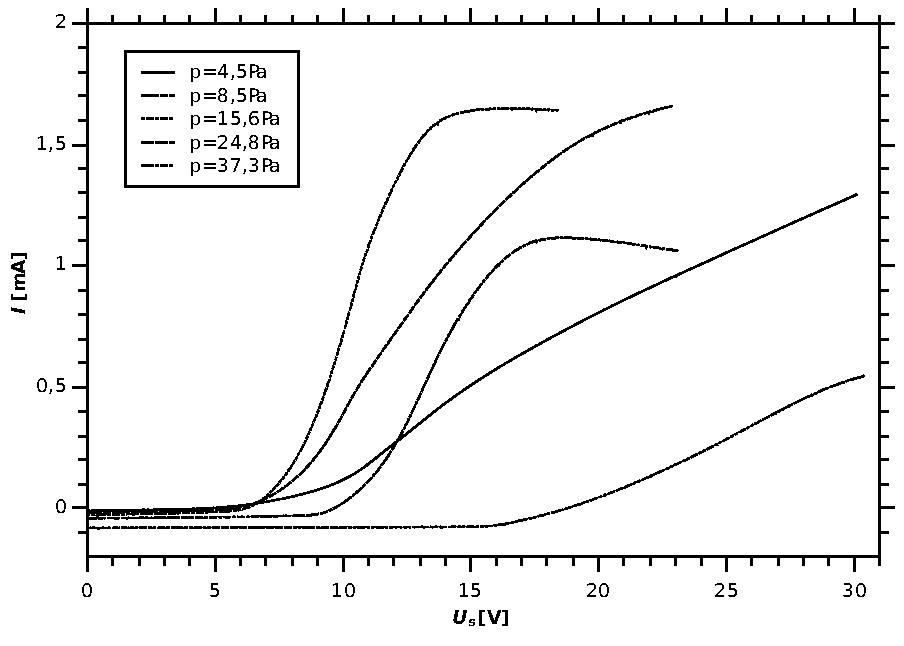
\includegraphics[width=12.8cm]{img/prubeh.pdf}
\caption{VA charakteristika sondy pro různé tlaky}
\label{VA}
\end{center}
\end{figure}

\subsection{Plovoucí potenciál}
Plovoucí potenciál $U_\mathrm{f}$ byl určen přímým odečtem z VA charakteristiky, je to napětí při kterém je celkový proud nulový.

\begin{table}[htbp]
\begin{center}
\begin{tabular}{|c|c|c|c|c|c|c|c|c|c|c|}
\hline
$p$\,[Pa] & 37,3 & 30,3 & 24,8 & 19,8 & 15,6 & 12,9 & 10,9 & 8,5 & 6,6 & 4,5 \\ \hline
$U_\mathrm{f}$\,[V] & 18,79 & 14,69 & 9,66 & 7,23 & 6,24 & 5,82 & 5,65 & 5,79 & 5,88 & 4,97
 \\ \hline
\end{tabular}
\caption{Plovoucí potenciál}
\label{}
\end{center}
\end{table}

\begin{figure}[htbp]
\begin{center}
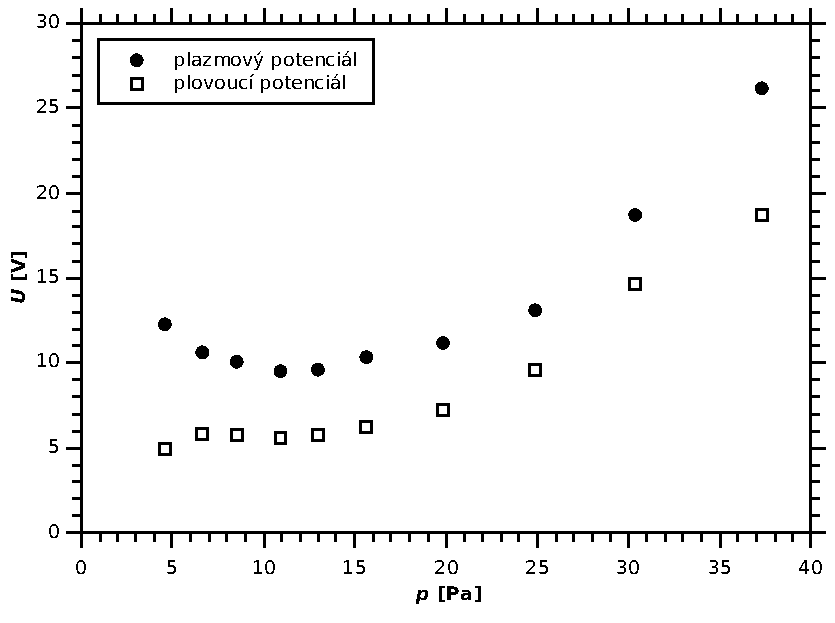
\includegraphics[width=12.8cm]{img/ufupl.pdf}
\caption{Plazmový a plovoucí potenciál v závislosti na tlaku}
\label{ufupl}
\end{center}
\end{figure}

\subsection{Plazmový potenciál}
Plazmový potenciál byl určen podle druhé derivace sondového proudu. Je to napětí, kde je druhá derivace nulová. Pro provedení derivace byl použit program derivace.m, s parametrem vyh=50, který v každém bodě VA charakteristiky nafitoval na oblast 2*vyh+1 bodů, se středem v daném bodě, parabolu. Dvojnásobek kvadratického členu paraboly je potom druhá derivace v daném bodě.

\begin{table}[htbp]
\begin{center}
\begin{tabular}{|c|c|c|c|c|c|c|c|c|c|c|}
\hline
$p$\,[Pa] & 37,3 & 30,3 & 24,8 & 19,8 & 15,6 & 12,9 & 10,9 & 8,5 & 6,6 & 4,5 \\ \hline
$U_\mathrm{p}$\,[V] & 26,2 & 18,76 & 13,17 & 11,2 & 10,37 & 9,64 & 9,55 & 10,1 & 10,74 & 12,32 \\ \hline
\end{tabular}
\caption{Plazmový potenciál}
\label{plptable}
\end{center}
\end{table}

\subsection{Odečet iontového proudu}
Dalším krokem při analýze proudu sondou a získání rozdělovací funkce elektronů je odečet iontového proudu. Toto se provádí nafitováním funkce $I = I_0 \left(1 + \frac{e(U_\mathrm{pl} - U_\mathrm{s})}{k T_\mathrm{e}}\right)^\kappa$ na oblast čistě iontového proudu (byl použit program ion\_current.m).  Obrázek \ref{ionparameters} shrnuje nafitované hodnoty iontového proudu.

\begin{figure}[htbp]
\begin{center}
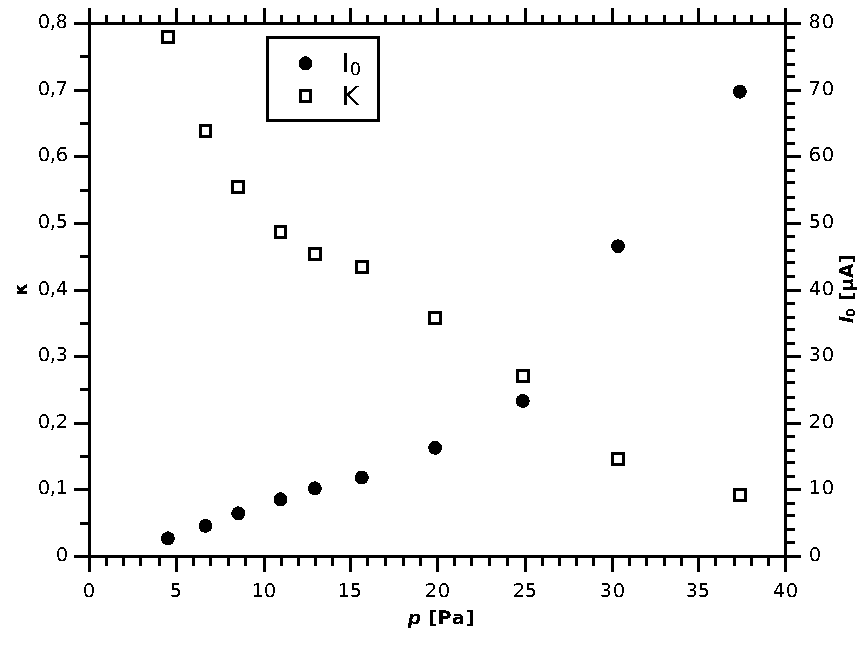
\includegraphics[width=12.8cm]{img/ionts.pdf}
\caption{Parametry iontového proudu v závislosti na tlaku}
\label{ionparameters}
\end{center}
\end{figure}

Po odečtení iontového proudu lze přistoupit k~analýze elektronové rozdělovací funkce. Pokud je funkce Maxwellova, měla by po zlogaritmování elektronového proudu být oblast těsně pod potenciálem plazmatu přibližně lineární. Ukázalo se, že oblast lineární není, proto byla následně spočítána druhá derivace elektronové rozdělovací funkce a z ní Druvensteinovou formulí určena experimentální rozdělovací funkce. Druhé derivace elektronového proudu jsou na obrázku \ref{secderiv}.

\begin{figure}[htbp]
\begin{center}
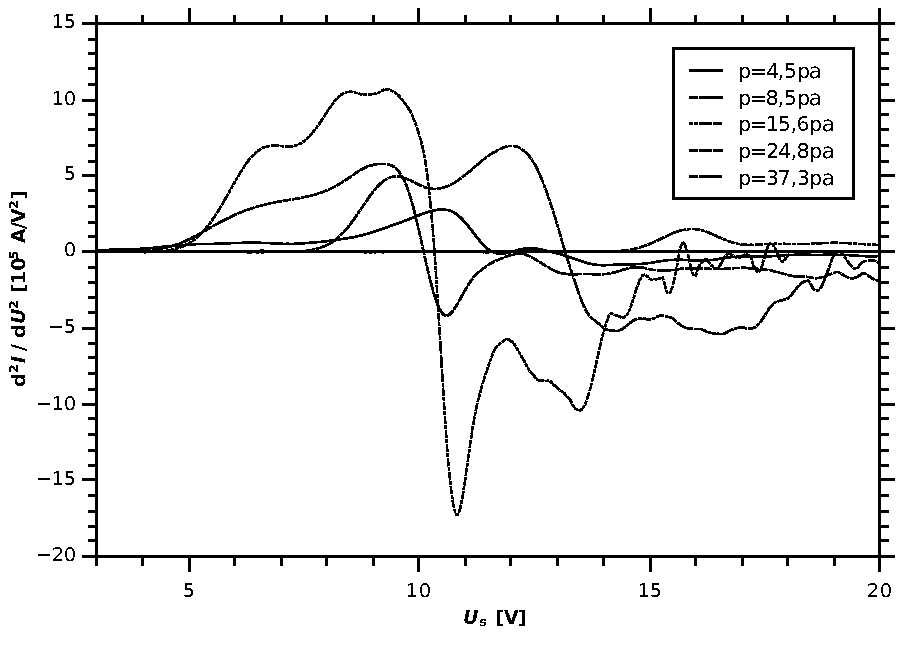
\includegraphics[width=12.8cm]{img/secderiv.pdf}
\caption{Průběh druhých derivací proudů sondou podle napětí pro různé tlaky}
\label{secderiv}
\end{center}
\end{figure}

\subsection{Rozdělovací funkce elektronů}
Rozdělovací funkce byly určeny pomocí Druyvesteinovy formule, jejich průběh je na obrázku \ref{rozdelfunc}.

\begin{figure}[htbp]
\begin{center}
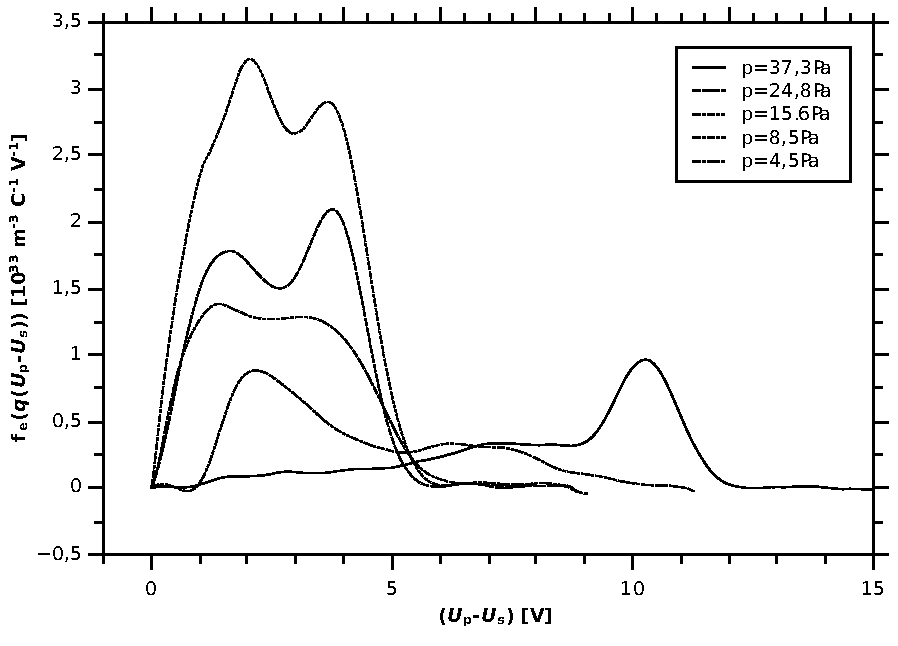
\includegraphics[width=12.8cm]{img/rozdelfunc.pdf}
\caption{Průběh experimentálních elektronových rozdělovacích funkcí pro různé tlaky}
\label{rozdelfunc}
\end{center}
\end{figure}

\subsection{Teplota a koncentrácia elektrónov}

Koncentrace a střední energie elektronů byly vypočítány integrály z rozdělovací funkce

\begin{equation}
n_\mathrm{e} = \int_{-\infty}^{U_\mathrm{p}} f(q(U_\mathrm{p}-U_\mathrm{s}))\,q\,dU_\mathrm{s}
\end{equation}

\begin{equation}
<E> =  \frac{1}{n_\mathrm{e}} \int_{-\infty}^{U_\mathrm{p}}\,q^2\,(U_\mathrm{p}-U_\mathrm{s})\,f(q(U_\mathrm{p}-U_\mathrm{s}))\, dU_\mathrm{s}
\end{equation}

Teplota (přestože není pro jiné než Maxwellovo rozdělení definovaná) byla poté spočítána jako $T = \frac{2<E>}{3 k}$. Hodnoty teploty a koncentrace elektronů pro různé tlaky v reaktoru jsou na obrázku \ref{final}.

\begin{figure}[htbp]
\begin{center}
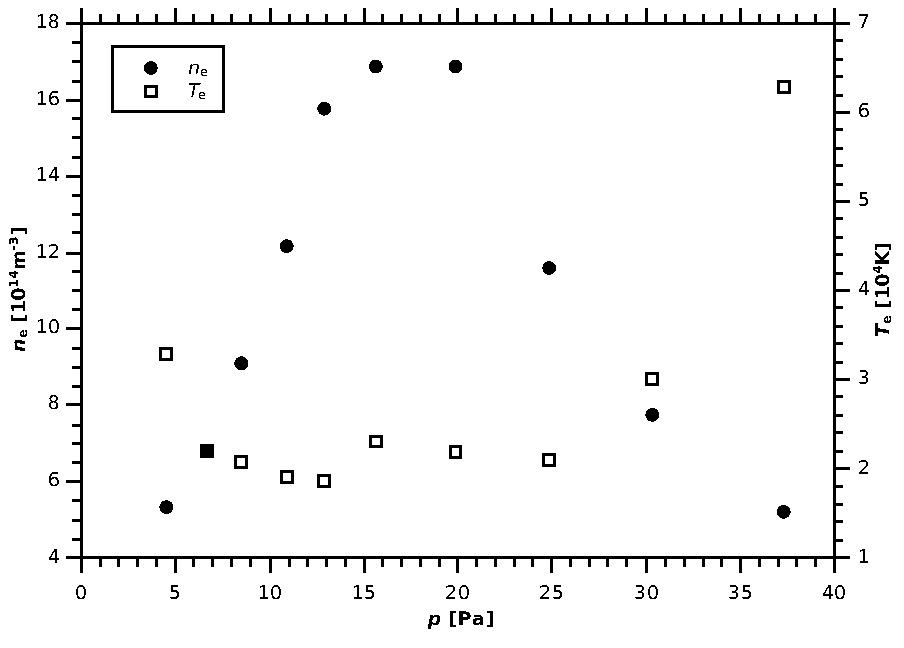
\includegraphics[width=12.8cm]{img/final.pdf}
\caption{Závislost elektronové teploty a koncentrace na tlaku}
\label{final}
\end{center}
\end{figure}

\subsection{Nekompenzovaná sonda}
Posledním měřením byla nekompenzovaná sonda, což je v podstatě jen drátek vložený do plazmatu. Na obrázku \ref{nekomp} můžeme vidět vznik vyšších harmonických frekvencí v plazmatu.

\begin{figure}[htbp]
\begin{center}
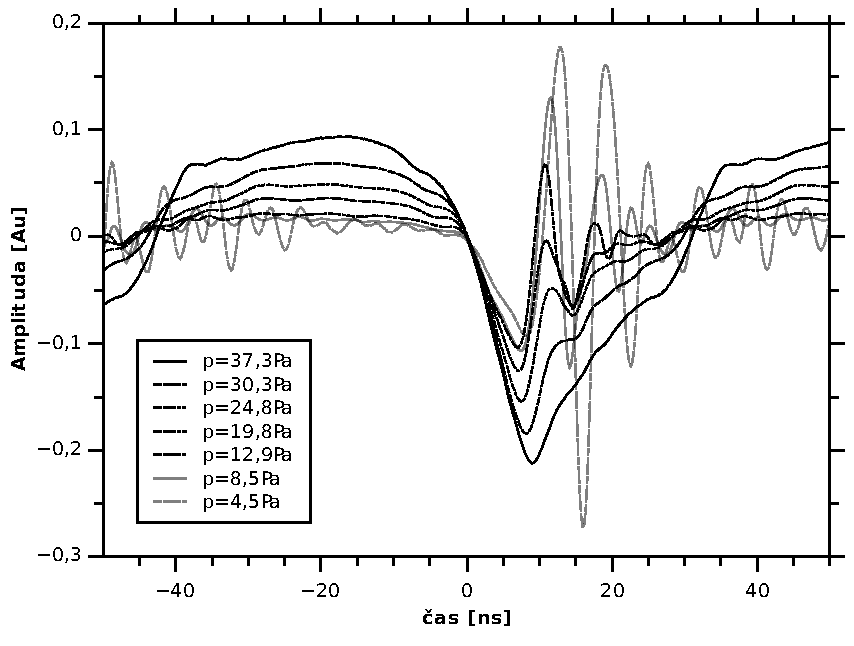
\includegraphics[width=12.8cm]{img/nekomp.pdf}
\caption{Nekompenzovaná sonda}
\label{nekomp}
\end{center}
\end{figure}


\section{Závěr}
V průběhu praktika byly naměřeny VA charakteristiky Langmuirovy sondy pro 10 různých hodnot tlaku v reaktoru, ve kterém hořel výboj v dusíku. Data byla následně vyhodnocena a byl určen plovoucí potenciál, plazmový potenciál, teplota a koncentrace elektronů. Také byly určeny některé konstanty iontového proudu. Ukázalo se, že plovoucí potenciál roste s  tlakem. Teplota elektronů a plazmový potenciál mají minimum v oblasti cca 10--15\,Pa. Koncentrace elektronů je naopak v tomto rozmezí tlaků maximální. Tato závislost teploty a koncentrace je způsobena tím, že byl po celou dobu měření výkon konstantní, tj. při větší elektronové koncentraci je energie připadající na jeden elektron menší. Rozdělovací funkce elektronů vykazují zajímavý ,,dvojhrbol'' , dle mého názoru se jedná o chybu vzniklou při derivaci, neboť ne na celé oblasti lze VA charakteristiku vhodně fitovat parabolou, až na tento rozdíl se rozdělovací funkce, zvlášť pro nižší tlaky, velmi podobají Maxvellově rozdělovací funkci. Také je zajímavé, že výsledné teplota elektronů (určená integrováním rozdělovací funkce) se mnohdy jen minimálně lišila od prvního odhadu elektronové teploty použitém při odečtu iontového proudu (například pro tlak 37,3\,Pa byl rozdíl menší než 5\,\%). Při analýze iontového toku se podle očekávání ukázalo, že $I_0$ s tlakem roste (protože roste koncentrace) a že $\kappa$ s tlakem klesá (s rostoucím tlakem srážky více ovlivňují iontový proud). V případě nekompenzované sondy můžeme vidět, že vyšší harmonické frekvence se v plazmatu projevují až s klesajícím tlakem. Nicméně již při vysokých tlacích dochází k~modulaci amplitudy od očekávané sinusoidy.

\end{document}
